%% Template for a preprint Letter or Article for submission
%% to the journal Nature.
%% Written by Peter Czoschke, 26 February 2004
%%

\documentclass{nature}
\usepackage{epsfig}
\usepackage{epsf}
\usepackage{pdflscape}
\usepackage{soul}
\usepackage{graphicx}
\usepackage{mathabx}
\usepackage{epstopdf} %converting to PDF
\usepackage{hyperref}
\usepackage[labelfont=bf]{caption}

\usepackage{natbib}
\setcitestyle{authoryear,open={(},close={)}}

%% make sure you have the nature.cls and naturemag.bst files where
%% LaTeX can find them

\title{Late Holocene structural style and seismicity of highly transpressional faults in southern Haiti}

%% Notice placement of commas and superscripts and use of &
%% in the author list

\author{Jiannan Wang, Paul Mann, Robert R. Stewart \\
\small All at: Department of Earth and Atmospheric Sciences, University of Houston, Houston, Texas, USA.}
%% \author{Jiannan Wang$^{1}$, Paul Mann $^{1}$, Robert R. Stewart $^{1}$}

\begin{document}

\maketitle

%\begin{affiliations}
%% \item Put institutions in this environment and
%% \item separate with \verb|\item| commands.
% \item Department of Earth and Atmospheric Sciences, University of Houston, Houston, Texas, USA.
%\end{affiliations}

\begin{abstract}
The devastating 2010 Haiti earthquake ($M_w$ 7.0) was caused by rupture of the L\'eog\^ane blind thrust fault located 5 km north of the main Caribbean-Gon\^ave plate boundary, the 1200 km-long, left-lateral Enriquillo-Plaintain Garden fault zone (EPGFZ). Unexpectedly, the EPGFZ remained largely quiescently although it formed the southern edge of the coseismic uplift and maximum ground shaking zone. Here, we use high-resolution sonar data from two Haitian lakes that straddle the EPGFZ to demonstrate the presence of a 10-15 km-wide, 120 km-long, late Holocene fold-thrust belt adjacent to the northern edge of the EPGFZ. Sonar results from Lake Azuey show that the EPGFZ is more deeply buried and less active than the adjacent, newly discovered, obliquely oriented thrust-fold belt. In Lake Mirago\^ane, our sonar survey identified the main, active strands of the EPGFZ bounding a deep pull-apart basin that has been active for at least the last 10 ka and possibly up to 50 ka, yet remains unaffected by the 2010 fault rupture and shaking. We interpret folding and thrusting along the northern edge of the EPGFZ that includes the devastating 2010 rupture of the L\'eog\^ane blind, thrust fault an manifestation of a highly transpressional EPGFZ fault system. In this fault system, coseismic deformation alternates at recurrence intervals of centuries between oblique shortening structures like the L\'eog\^ane thrust and strike-slip rupture of the main EPGFZ.
\end{abstract}

On 12 January 2010, a $M_w$ 7.0 earthquake struck the densely populated Port-au-Prince region of south-central Haiti and caused widespread destruction with more than 200,000 fatalities and an estimated 8 billion dollars damage  \citep{prentice2010seismic,kocel2016near}. 
Integrated field observations of coastal uplift  \citep{hayes2010complex,hashimoto2011fan}, remote sensing and radar interferometry  \citep{cowgill2012interactive}, Global Positioning System (GPS) geodesy and modeling \citep{calais2010transpressional,hayes2010complex,prentice2010seismic,symithe2013coseismic,douilly2013crustal,douilly2015three}, and aftershock studies \citep{calais2010transpressional,hayes2010complex,douilly2013crustal,douilly20163d} all indicated that the earthquake ruptured a previously unrecognized and deeply-buried, onshore fault - the L\'eog\^ane thrust fault - and a previously recognized, offshore fault - the Trois Baies thrust fault \citep{mercier20112010,symithe2013coseismic}. These two, 8 and 20 km-long thrusts, obliquely trending at angles of $8^{\circ}$ and $20^{\circ}$, respectively, to the adjacent left lateral strike-slip plate boundary between the Caribbean plate and the Gon\^ave microplate \citep{mann1995actively,calais2010transpressional,benford2012gps}, the Enriquillo-Plantain Garden fault zone (EPGFZ), moved without accompanying slip \citep{calais2010transpressional,hayes2010complex,prentice2010seismic} on the geomorphically prominent EPGFZ, located only 1-5 km to the south (Figure \ref{figure1}A). Quantified by GPS measurements \citep{calais2010transpressional}, the remarkably large angle ($45^{\circ}$-$55^{\circ}$) of obliquely convergent plate motion across the EPGFZ (Figure \ref{figure1}) indicates that this region of the EPGFZ is the most transpressional zone of the northern Caribbean strike-slip boundaries \citep{mann2002oblique} -- and one of the most transpressional for any strike-slip plate boundary worldwide \citep{mann2007overview}.  

The broad, 250 km-wide zone of transpression spanning the entire width of the island of Hispaniola is driven by oblique motion between the North America, Caribbean, and Gon\^ave plates and includes: 1) the highest topography, up to 3 km in the northern Caribbean region; 2) strain partitioning along the EPGFZ and the subparallel Septentrional strike-slip fault zone along the north side of the island as known from GPS studies \citep{calais2010transpressional,hayes2010complex,prentice2010seismic,symithe2013coseismic,douilly2013crustal,douilly2015three}; 3) left-lateral strike-slip rupture of the EPGFZ in the 18th century inferred from historical earthquakes \citep{prentice2010seismic}; and 4) folding and thrusting of 10-15 km-wide belt of Miocene to Quaternary rock adjacent to the EPGFZ \citep{saint2015seismotectonics}.

Coseismic deformation along a large transpressional strike-slip fault, such as the EPGFZ or the San Andreas fault zone in California \citep{segall1990surface}, either is accommodated on the main fault, which may eventually trigger major earthquakes, or is accommodated by oblique, secondary structures adjacent to the main fault, which may spare coseismic rupture on the main fault for longer periods. Highly transpressional areas like Hispaniola can lead to the generation and increased activity on more favorably and obliquely oriented folds and thrusts whose coseismic rupture might alternate with much longer ruptures along the adjacent strike-slip fault. For the EPGFZ region, the oblique thrusts spaced at distances of 1-8 km along the main strike-slip fault, obliquely intersect the main strike-slip fault at angles of $30^{\circ}-45^{\circ}$ and trend northeastward away from the central fault. As a result of this geometry, earthquake rupture initiating on an oblique thrust like the L\'eog\^ane fault is likely confined to that vicinity and may not connect with other oblique thrusts or the main strike-slip faults \citep{douilly2015three}.

The distribution of complex Holocene folding and thrusting in the 10-15 km wide zone of deformation is mirrored in the pattern of coseismic and vertical deformation recorded by Interferometric Synthetic Aperture Radar (InSAR) \citep{hashimoto2011fan} (Figure \ref{figure2}A). The wavelengths of folds linked to oblique thrusts, vary from 1 to 8 km and deform Miocene and younger fine to coarse-grained, basinal, and coastal plain rocks in the belt 10-15 km wide and parallel to the EPGFZ. These folds in clastic lithologies contrast with longer wavelengths that have more continuous fold axes found in more massively bedded Cretaceous to Eocene rigid, basaltic, and carbonate lithologies exposed at south of the EPGFZ (Figure \ref{figure2}B). InSAR revealed that the 2010 earthquake elevated the smaller folds of the L\'eog\^ane fan-delta north of the EPGFZ, yet produced coseismic subsidence in the 1.4 km-high, less complexly deformed, mountain range south of the EPGFZ to the south \citep{hashimoto2011fan} (Figure \ref{figure2}A). Despite the proximity (around 5 km) of the L\'eog\^ane thrust fault and its neighboring EPGFZ, the EPGFZ unexpectedly remained largely quiescently outside the zone of 2010 coseismic uplift and maximum ground shaking \citep{nettles2010earthquake}. The centroid moment tensor (CMT) mechanism shows a primarily strike-slip motion, with a small component of reverse motion, on a steeply north-dipping nodal plane \citep{nettles2010earthquake,douilly2013crustal}. Finite element modeling \citep{douilly2015three} suggests that L\'eog\^ane fault in the basinal area absorbs most of the energy of the northwest-southeast compression on the obliquely-striking, high-angle ($30^{\circ}-45^{\circ}$) reverse fault planes, leaving significantly increasing but insufficient stress to trigger slip on the adjacent EPGFZ (Figure \ref{figure2}A).

This paper integrates geophysical and geological observations from the 2010 earthquake epicentral region of Haiti to better define the nature of the late Holocene transpressional deformation within the 10-15 km-wide but laterally persistent band of the low-relief, inland Cul-de-Sac basin and the coastal plain areas. This belt of deformation along the northern edge of the EPGFZ is overlain by the Lakes Mirago\^ane, Azuey in Haiti and Lake Enriquillo in the neighboring country of Dominican Republic (Figure \ref{figure1}B). To describe structures related to both the EPGFZ and its flanking belt to the north, a total of 94 km of high-resolution (2-10 kHz) sonar profiles were collected in 2014 from the 129 km\textsuperscript{2}, brackish Lake Azuey and 37 km of profiles from the 14 km\textsuperscript{2}, fresh-water Lake Mirago\^ane. The EPGFZ strikes approximately west-east, so 80\% of our grid on Lake Azuey and 90\% of our grid on Lake Mirago\^ane was dedicated to the north--south profiles. The average speed of the boat towing the sonar was 3 knots, and we used a sonar pulse rate of 4 per second. Our 2--10 kHz sonar frequency range gives sub-bottom layer resolution of about 10 cm. These surveys were the first sonar surveys in Haitian lakes. Both lakes straddle the active trace of Haiti's EPGFZ and its adjacent, transpressional fold-thrust belt, therefore provide constraints on the location, structural style, and timing of deformation within both structural provinces (Figure \ref{figure2}B).

Based on both of our lake surveys combined with a previous survey of Lake Enriquillo in the Dominican Republic \citep{rios2013holocene} and the previous geologic mapping of the basinal and topographic corridor of the Cul-de-Sac basin in Haiti and the Enriquillo basin in the Dominican Republic \citep{mann1995actively,mann1999caribbean}, a first-order question we pose is whether the EPGFZ extends as a continuous, strike-slip fault along the 120 km-long zone of deformation of Miocene and younger clastic rocks present between the two lakes (Figure \ref{figure1}B). Previous studies  \citep{saint2015seismotectonics,symithe2016present} have proposed that the EPGFZ terminates as a strike-slip feature in the area south of Port-au-Prince; these studies further propose that transpressional plate motion in the eastern Cul-de-Sac basin, and the Enriquillo Valley in the Dominican Republic is entirely accommodated along the low-angle, oblique-thrust structures that overthrust the southern edges of Lake Azuey and Lake Enriquillo (Figure \ref{figure1}B).   

In the Lake Azuey area, we mapped a linear and east-west striking fault trace in deformed Holocene sediments along with its landfall. Integrated with previous land mapping of the EPGFZ \citep{mann1995actively,prentice2010seismic,cowgill2012interactive}, we interpret this linear east-west striking feature in Lake Azuey as a 5-30 meter-wide and continuous trace of the EPGFZ which we can follow eastward to the EPGFZ locality at Dumay, about half way between Lake Azuey and Port-au-Prince, which was previously described and dated as a 6 m offset of a stream channel \citep{cowgill2012interactive} (shown in Figure \ref{figure2}A). The structural cross sections in this area taken from previous studies \citep{massoni1955haiti,mann1995actively,douilly2015three} indicate that the high-angle EPGFZ co-exists with adjacent thrusts over-thrusting from the south and north (Figure \ref{figure2}C,D). Sonar profiles from the southernmost area of Lake Azuey (Figure \ref{figure2}C,D) show that the most recent rupture of the EPGFZ is covered by about 0.7 m of Holocene sediment, suggesting that there has been no recent activity of the EPGFZ. We project this trace of the EPGFZ along a prominent fault valley at the town of Jimani that separates Lakes Azuey and Enriquillo (Figure \ref{figure2}B). A previous study of Lake Enriquillo \citep{rios2013holocene} identified the break along the northeastern edge of Cabritos Island in Lake Enriquillo which aligns exactly with the large east-western lineament extending eastward from our map area in Lake Azuey (Figure \ref{figure2}B). For this reason, we conclude that this linear, late Holocene strike-slip fault extends at 55 km to, at least, to the eastern edge of Lake Enriquillo where the recently documented uplift of the Holocene reef fringes Lake Enriquillo \citep{mann1995actively}.  
%The cross-sections (Figure \ref{figure2}D) from this and previous work \citep{massoni1955haiti,douilly2015three} indicate that the secondary fault-thrusts have a similar orientation as the north-dipping thrust on the north side of the EPGFZ. This orientation, about $30^{\circ}$ to the EPGFZ, suggests the secondary faults have the same type of ``off axis'' deformational mechanism. All three faults appear to be more active than the EPGFZ. The wide-spread distribution of such active secondary structures suggests that the stress is released more frequently through the secondary faults than by the main fault, which further supports the high-friction deformational mechanism of the EPGFZ.

A second basic question is the age of the EPGFZ and its adjacent zone of fold-and-thrust deformation, and the age of the deformed sediments observed on sonar profiles from Lakes Azuey and Enriquillo. Both previous coring in Lake Enriquillo \citep{rios2013holocene}, which was tied to onshore stratigraphic studies \citep{taylor1985stratigraphy,rios2013holocene}, and in Lake Mirago\^ane \citep{higuera199910} have established the late Holocene to include the upper 5 and 7 meters of both lakes, respectively. In Lake Enriquillo, a sonar survey similar to ours was conducted in 2013 \citep{rios2013holocene}. The sonar events, which are interpreted as stratigraphic features, from Lake Azuey and Lake Enriquillo (Line B1 and Line L19 in Figure \ref{figure2}F) correlate convincingly (Figure \ref{figure2}F). Given the small distance separating the two lakes ($\sim$4 km); the similarity of the stratigraphic profiles; and the same amount of sediment above the EPGFZ; it is reasonable to suggest that Lake Azuey and Lake Enriquillo share the same sedimentation history as well as the same structural style and seismicity related to the EPGFZ and its oblique, thrust faults.

The EPGFZ in both Lake Enriquillo and Lake Azuey is buried by 0.7 m of sediments. According to coring studies in the Dominican Republic \citep{taylor1985stratigraphy,rios2013holocene}, the 5.2 m thickness of the latest lake stage (2 ka BP to present) gives a recent Holocene average sedimentation rate of 2.6 mm/yr. Using the average sediment rate, the most recent rupture of the EPGFZ would be dated some 270 years ago. Given the historical earthquake records \citep{bakun2012significant}, we suggest that the most recent rupture of the EPGFZ is October or November of 1751, and the deformed sediments in Lake Azuey are Holocene age (Figure \ref{figure2}C,D). 
%
%A sonar survey similar to ours was conducted in 2013 in the adjacent Lake Enriquillo in the Dominican Republic \citep{rios2013holocene}, some 4 km east of Lake Azuey (Figure \ref{figure1}B). We compared sonar profiles acquired from Lake Azuey and Lake Enriquillo (Line B1 and Line L19 in Figure \ref{figure2}F). The sonar events interpreted as stratigraphic features in the two lakes, correlate convincingly (Figure \ref{figure2}F). Using the stratigraphic information extrapolated from Lake Enriquillo, all of the sediments deformed by the EPGFZ and Jimani fault in Figure \ref{figure2}C,D would be Holocene in age. 
%The EPGFZ in both Lake Enriquillo and Lake Azuey is buried 0.7 m beneath sediments. Given the lakes' proximity, the similarity of the stratigraphic profiles, and the same amount of sediment above the EPGFZ, it is reasonable to suggest that Lake Azuey and Lake Enriquillo share the same sedimentation history as well as seismicity. According to coring studies in the Dominican Republic \citep{taylor1985stratigraphy,rios2013holocene}, the 5.2 m thickness of the latest lake stage (2 ka BP to present) gives a recent Holocene average sedimentation rate of 2.6 mm/yr. Using the average sediment rate, the most recent rupture of the EPGFZ would be dated to around 1745. Considering the historical earthquake records \citep{bakun2012significant}, we suggest that the most recent rupture of the EPGFZ is October or November of 1751.

A third tectonic question is the source of the folding observed in the 10-15 km-wide belt along the EPGFZ (Figure \ref{figure2}A,B). On a more regional scale (Figure \ref{figure2}A), the oblique folds and faults in the Lake Azuey area form part of continuous series of \textit{en echelon}, contractional structures along the EPGFZ which curve into parallelism with the EPGFZ. A previous hypothesis is that the Haitian fold-and-thrust belt described in the range north of the Cul-de-Sac Valley \citep{pubellier2000plate} propagated southwestwards from the Miocene to present-day and became emergent as anticlinal hills protruding on the alluvial plain along the southern edge of the Cul-de-Sac valley \citep{calais2010transpressional}. Another previous study proposed that folding along the EPGFZ was a consequence of overlapping the main traces of the EGPFZ \citep{cowgill2012interactive}. 

In Lake Azuey north of the EPGFZ, we discovered an oblique fold that deforms the Holocene lake sediments (Figure \ref{figure2}C,D) and overlies a north-dipping thrust fault, which we named the Jimani thrust fault. Differing from other parts of the lake, this fold has a very clear and strong reflection from its top, indicating that the fold is active. The trace of the Jimani thrust fault strikes about $30^{\circ}$ oblique to the EPGFZ (Figure \ref{figure2}A). 

Structural cross-sections (Figure \ref{figure2}E) from this and the previous works \citep{massoni1955haiti,douilly2015three} along this 120 km-long zone of deformation adjacent to the EPGFZ show that the oblique thrust faults share a similar orientation with other north-dipping thrusts along the northern edge of the EPGFZ. All three of these oblique thrust faults shown on the cross sections deform rocks as young as Pliocene and Quaternary \citep{saint2015seismotectonics}. In our sonar survey of Lake Azuey, we noted that the most prominent folds present adjacent to the EPGFZ become less prominent in the central and northern parts of the lake (Line C-C' in Figure \ref{figure2}E). These southern folds and thrusts imaged in Lake Azuey define the transpressive belt along the EPGFZ observed in onshore areas to the west (Figure \ref{figure2}A,B). A similar pattern of deformation is observed in Port-au-Prince Bay where the central and northern edge of the basin is undeformed \citep{massoni1955haiti,mchugh2011offshore,saint2015seismotectonics}. The structural trends and distinctive, sigmoidal shapes of these folds and their concentration along the southern edge of the Cul-de-Sac basin do not in our view support the idea that they represent the southward propagation of the fold-and-thrust belt from the mountains forming the northern edge of the Cul-de-Sac Valley as proposed by previous workers \citep{calais2010transpressional} (Figure \ref{figure2}A,B). 
%
%The cross-sections (Figure \ref{figure2}E) from this and previous work \citep{massoni1955haiti,douilly2015three} along a 50 km long zone of deformation indicate that the secondary fault-thrusts have a similar orientation as the north-dipping thrust on the north side of the EPGFZ. This orientation, about $30^{\circ}$ to the EPGFZ, suggests the secondary faults have formed in the 10-15 km-wide zone of thrusts and folds with all three faults deform rocks as young as Pliocene and Quaternary \citep{saint2015seismotectonics}.

The 2010 aftershock zone at the western and central part of our study area (Figure \ref{figure3}A) reflects rupture along the northwest-striking, 20-km-long, submarine, Trois Baies thrust fault that forms the western extension of the 10-15 km-wide, transpressional zone north of the EPGFZ. As the Trois Baies fault is submarine, InSAR cannot be used to assess its 2010 coseismic similarity with folding and thrusting affected the onshore, L\'eog\^ane plain. However, the same basic structural elements of the L\'eog\^ane plain are also observed for the Trois Baies thrust fault that include the short distance (1 km) to the EPGFZ, and its steep ($45^{\circ}$) but opposite, southwest dip of the Trois Baies thrust fault (Figure \ref{figure3}A). One of the most intense zones of coseismic, aftershock, and coastal uplift separates the oppositely-dipping L\'eog\^ane and Trois Baies faults and may represent complex, deformation at a transfer zone between the two faults (Figure \ref{figure3}A). The aftershock study of the Trois Baies fault \citep{symithe2016present} shows that it is comparable to the cross sections of the eastern area in Figure \ref{figure2}E. The overall structure of this western part of the study area (Figure \ref{figure3}A) mirrors the same geometry of oblique thrusts and the main EPGFZ described from the eastern part of the study area (Figure \ref{figure2}A).

In the onshore part of the western study area, Lake Mirago\^ane was interpreted as a 14 km\textsuperscript{2} pull-part basin developed as a left-stepping, releasing bend on the EPGFZ paired with the adjacent Tapion Du Petit Go\^ave restraining bend 12 km to the east \citep{cowgill2012interactive}. Bathymetry from our sonar data shows the maximum water depth of Lake Mirago\^ane is 42.8 m (Figure \ref{figure3}B), which makes this actively faulted lake the deepest \citep{higuera199910} in the Caribbean region. The 30 m of recognizable stratigraphy (Figure \ref{figure3}C,D) from the sonar survey in Lake Mirago\^ane reveals a series of deformational features including major east-west normal faults, minor thrust faults at deep (some 20 m), and active folds at the lake bottom (Figure \ref{figure3}B and Figure \ref{figure3}C,D). The upper 7 m of the lake was cored and dated as 10 ka at the bottom of the core. Extrapolating the sedimentation rate to the observed thickness of 30 m in the lake allows a minimum of 33 ka to be calculated for the age of the pull-apart basin on the EPGFZ. Core measurements of the E/P (evaporation and precipitation ratio from the $\delta^{18}$O of ostracod shells in the core sample) were undertaken \citep{higuera199910} in the center of Lake Mirago\^ane (Figure \ref{figure3}B). The core reveals the uppermost part of the sediment is Holocene and the latest Pleistocene lacustrine (Figure \ref{figure3}E). Pollen data from the core indicate alternating dry and wet environments. Comparing the core data with the sonar data, we can see the sediment layers from drier climates (higher E/P) correlate with stronger acoustic reflectivity and vice versa (Figure \ref{figure3}E). We applied a low-pass filter on the pollen log data and found a strong correlation between the pollen and sonar data (red curve in Figure \ref{figure3}F). To further investigate this interesting correlation between the geochemical and geophysical data, we use the filtered E/P log, considered as pseudo-acoustic impedance log, to generate a synthetic sonar response (Figure \ref{figure3}F). The correlation is compelling which suggests that the depositional environment influences the acoustic properties of the sediments and sonar response may be a partial proxy for climatic processes. Considering the historical document record \citep{bakun2012significant}, the dating of the core and sonar interpretation in Lake Mirago\^ane suggest that the most recent rupture in this lake is likely related to a historic earthquake in 1770 \citep{bakun2012significant}.

In summary, our lake studies, along with previous work, favor a model of a 10-15 km wide transpressional zone that deforms thick, loosely-consolidated, Miocene to recent clastic rocks in coastal, marine, and lake settings as shown in three dimensions (Figure \ref{figure4}). Moving from Lake Azuey in the east to the west, the block diagram illustrates along-strike changes observed in the dips of the thrust faults and obliquely orientation to the EPGFZ. Fold axes north of the EPGFZ range from 3 to 20 km in length and are sigmoidally related to the EPGFZ in map view (Figure \ref{figure2}B). Dip direction and amounts on these thrust faults vary from north-dipping at $21^{\circ}$ on the Jimani fault (Figure \ref{figure2}E, Figure \ref{figure4}), south-dipping on the Lamentine fault \citep{saint2015seismotectonics} at $40^{\circ}$, north-dipping at $70^{\circ}$ on the L\'eog\^ane fault active during the 2010 earthquake (Figure \ref{figure2}E, Figure \ref{figure4}), and south-dipping on the Trois Baies fault at $45^{\circ}$ (Figure \ref{figure4}). South of the EPGFZ, transpressional folding in more rigid Cretaceous basalts and overlying Eocene limestone have wavelengths ranging from 1 to 8 km. InSAR images of the 2010 earthquake indicate smaller folds and more seismogenic deformation in the 10-15 km belt north of the EPGFZ as opposed to the broader folding and less seismogenic deformation south of the EPGFZ. 

We propose that the folds north of the EPGFZ formed originally as conjugate thrust faults, reflecting the northeast to southwest convergence indicated by GPS vectors and highly transpressional character of the EPGFZ \citep{calais2010transpressional}. Conjugate thrust faults are common in thick sedimentary basins undergoing active shortening, as documented in the Chi-Chi Taiwan earthquake in 1999 \citep{chen2002conjugate}. Aftershocks north of the EPGFZ reflect the most recent phase of NE-SW shortening on the $70^{\circ}$ dipping reverse fault planes \citep{nettles2010earthquake}, along the deeply buried L\'eog\^ane thrust fault, as shown in the cross section in Figure \ref{figure2}E. These aftershocks define a conjugate pair of reverse faults with the dominant motion on the north-dipping fault plane. In the areas of high sedimentation rate such as the L\'eog\^ane plain, the thrusts are buried to a depth of about one km \citep{kocel2014searching}. In areas of lower sedimentation rate, the faults and folds are emergent at the surface or shallowly buried (Figure \ref{figure2}B). Because of the soft, unconsolidated material north of the fault, erosion rates are faster, and co-seismic uplifts are transitory and quickly reduced by erosion. While the oblique thrust planes form smaller fault segments ranging in length from 3 to 11 km (\ref{figure2}A,B), the 2010 earthquake demonstrates that oblique thrusts like the L\'eog\^ane fault are capable of producing a $M_w$ 7.0 earthquake with devastating results especially when coupled with inadequate construction practices \citep{symithe2016present}.

Paleoseismic estimates of the age of the most recent deformation of Lake Azuey, eastern Haiti, suggests that the latest activity of the EPGFZ in this area was in 1751 \citep{prentice2010seismic,bakun2012significant}. Similar analysis indicates that the latest earthquake event in the Lake Mirago\^ane area, western Haiti, was in 1770 \citep{bakun2012significant}. This suggests the earthquake recurrence cycle along the EPGFZ is about 250 years. Therefore, in this transpressional setting, the earthquake cycle may consist of an interplay between ruptures on the EPGFZ and ruptures on the oblique thrusts and related folds. The 2010 $M_w$ 7.0 earthquake released part of the stress of the region, but as the oblique thrusts may not be directly linked to the EPGFZ, it is possible that stresses on the EPGFZ have continued to accumulate since the 18th century \citep{prentice2010seismic}. Integrated paleoseismic study of the EPGFZ with the commonly buried oblique thrust faults, using geophysical and geologic methods, can help to inform the critical social issue of how future earthquakes will be partitioned between the larger EPGZ and other more obscure, oblique faults.

%On the west side of the Hispaniola, the left-lateral strike-slip EPGFZ develops into a left-stepping rhomboidal pull-apart feature, the Mirago\^ane Basin \citep{mann1983development,prentice2010seismic}. Fresh-water Lake Mirago\^ane straddles the trace of the EPGFZ (Figure \ref{figure3}A). Bathymetry from the sonar data shows the deepest part of Lake Mirago\^ane is 42.8 m (Figure \ref{figure3}B), which makes this lake the deepest \citep{higuera199910} in the Caribbean region. The 30 m of recognizable stratigraphy (Figure \ref{figure3}C,D) from the sonar survey in Lake Mirago\^ane reveals a series of deformational features including major east-west normal faults, minor thrust faults at deep (some 20 m), and active folds at the lake bottom (Figure \ref{figure3}B and Figure \ref{figure3}C,D).
%
%Aftershocks of the 2010 earthquake in the Mirago\^ane region occurred on a secondary south-dipping thrust fault, the Trois Baies thrust fault \citep{symithe2013coseismic,douilly2015three} (about $20^{\circ}$ to the north of the EPGFZ). In the Mirago\^ane basin itself, no evidence of active seismogenic rupture was found. However, there are some topographic subsidence, uplift, and fracture features with no lateral displacement (Figure \ref{figure3}C,D). The InSAR image indicates the displacement after the earthquake extended in the offshore area northeast of the L\'eog\^ane delta fan. Further investigation suggests that these discontinuities are due to gravity settling instead of fault activation \citep{prentice2010seismic,hayes2010complex}. In the sonar profiles, no obvious breaks extend to the surface. Several folds appear close to the normal faults, indicating that they are probably the result of gravitational sliding (Figure \ref{figure3}B).
%
%Core measurements of the E/P (evaporation and precipitation ratio from the $\delta^{18}$O of ostracod shells in the core sample) were undertaken \citep{higuera199910} in the center of Lake Mirago\^ane (Figure \ref{figure3}B). The core reveals the uppermost part of the sediment is Holocene and the latest Pleistocene lacustrine (Figure \ref{figure3}E). Pollen data from the core indicate a dry environment from 10,000 yr B.P to 7000 yr B.P. Comparing the core data with the sonar data, we can see the sediment layers from drier climates (higher E/P) correlate with stronger acoustic reflectivity, and vice versa (Figure \ref{figure3}E). We applied a low-pass filter on the pollen log data and found a strong correlation between the pollen and sonar data (red curve in Figure \ref{figure3}F). To further investigate this interesting correlation between the geochemistry and geophysics data, we use the filtered E/P log, consider it a pseudo-acoustic impedance log, and then generate a synthetic sonar response (Figure \ref{figure3}F). The correlation is compelling which suggests that the depositional environment has an influence on the acoustic properties of the sediments and sonar response may be a partial proxy for climatic processes. Historical documents record an earthquake occurred in 1770  \citep{bakun2012significant} in the area. The dating of the core and sonar interpretation in Lake Mirago\^ane suggest that the most recent rupture in this lake may well be due to the historic earthquake.
%
%The rupture of the secondary Trois Baies thrust fault, instead of the main fault strand, indicates that the secondary fault is more fragile. The east-west rupture direction of the 2010 earthquake \citep{hashimoto2011fan,douilly20163d} implies that the main fault was most likely locked and the oblique stress squeezed the formation toward the northwest direction (Figure \ref{figure4}). Gravitational sliding in this region during the earthquake may be a side-effect of the movement of the Trois Baies thrust fault. Considering the orientation of the Trois Baies thrust fault ($20^{\circ},$), we suggest that high friction locked the EPGFZ main fault strand, resulting in the rupture of the secondary fault. This hypothesis is consistent with the previous assessment of the L\'eog\^ane-Azuey area. In addition, the offshore geophysical survey in the western part of the Jamaica Passage suggests the compressional component of the EPGFZ is accommodated by pervasive multiple folds and thrusts close to the plate boundary rather than partitioned on the main bordering strike-slip faults  \citep{leroy2015segmentation,corbeau2016transpressive}. Combining all the evidence, we think in such transpressive tectonic setting, the plate boundary (EPGFZ) has high friction and secondary oblique faults are releasing the tectonic strain. 
%
%In summary, our lake studies, along with previous work, favor a model of high drag-distributed shear as the deformation mechanism of the EPGFZ with associated high-angle secondary faults. Paleoseismic consideration of Lake Azuey (eastern Haiti) suggest that the latest activity of the EPGFZ was in 1751 in the region. In addition, similar analysis indicates that the latest earthquake event in the Lake Mirago\^ane area was 1770. This suggests the earthquake cycle along the EPGFZ could be about 250 years. Therefore, in this transpressional setting, the earthquake cycle may consist of an interplay between ruptures on the high-friction main fault and ruptures on secondary thrusts and related folds. Even rupturing on the secondary faults can be devastating as evidenced by the severity of the 2010 event  \citep{mchugh2011offshore,kocel2016near}. This $M_w$ 7.0 earthquake released part of the stress of the region, but stresses are likely still accumulating. If the stress overcomes the frictional breakpoint along the main fault, energy release could be substantial. As the EPGFZ bisects the some of the most populated areas of Haiti and the Dominican of Republic, further attention to it is warranted.
%
%New add references  \citep{odonne1983analogue,mann1984subaerially,tikoff1998physical,calais2002strain,titus2007kinematic,mercier20112010,moknatian2017development}. 
%\section*{Another Section}
%
%Sections can only be used in Articles.  Contributions should be
%organized in the sequence: title, text, methods, references,
%Supplementary Information line (if any), acknowledgements,
%interest declaration, corresponding author line, tables, figure
%legends.
%
%Spelling must be British English (Oxford English Dictionary)
%
%In addition, a cover letter needs to be written with the
%following:
%\begin{enumerate}
% \item A 100 word or less summary indicating on scientific grounds
%why the paper should be considered for a wide-ranging journal like
%\textsl{Nature} instead of a more narrowly focussed journal.
% \item A 100 word or less summary aimed at a non-scientific audience,
%written at the level of a national newspaper.  It may be used for
%\textsl{Nature}'s press release or other general publicity.
% \item The cover letter should state clearly what is included as the
%submission, including number of figures, supporting manuscripts
%and any Supplementary Information (specifying number of items and
%format).
% \item The cover letter should also state the number of
%words of text in the paper; the number of figures and parts of
%figures (for example, 4 figures, comprising 16 separate panels in
%total); a rough estimate of the desired final size of figures in
%terms of number of pages; and a full current postal address,
%telephone and fax numbers, and current e-mail address.
%\end{enumerate}
%
%See \textsl{Nature}'s website
%(\texttt{http://www.nature.com/nature/submit/gta/index.html}) for
%complete submission guidelines.
%
%\begin{methods}
%The E/P (evaporation and precipitation ratio) log is acquired by measuring the $\delta^{18}$O of ostracod shells in the core sample \citep{higuera199910}. To find the analogical link between the geochemistry data (E/P log) and the geophysics data (sonar data), we applied a low-pass filter to the raw E/P log (Figure \ref{figure4}D). The E/P ratio variation has a strong correlation with the acoustic reflections, which relates to the acoustic impedance variation. 
%
%If we consider the E/P log as a pseudo-impedance log ($I(t)$), using the same source setting as the sonar (2-10 kHz linear sweep), we can generate the synthetic pseudo-acoustic reflections ($d_a$) as follow:
%\begin{eqnarray}
%{d_a}(t)=S(t) \Asterisk I(t),
%\label{analytic_equation}
%\end{eqnarray}
%where S(t) is the source signal. 
%In addition, the acoustic reflections ($d_a$) could be described as the analytic signal:
%\begin{eqnarray}
%{d_a}(t)=d(t)+iH[d(t)],
%\label{analytic_equation}
%\end{eqnarray}
%where H[d(t)] is the Hilbert transform of the real part of data, ${d_a}(t)$ is the analytic form of the data.
%
%To compare the synthetic pseudo-acoustic reflection data with the chirp sonar data, we compress the synthetic pseudo-acoustic reflection data: 
%\begin{eqnarray}
%E({d_a}(t))&=&\sqrt{Re[{d_a}(t)]^2+Im[{d_a}(t)]^2}\nonumber \\
%&=&\sqrt{d(t)^2+H[d(t)]^2},
%\label{evelop_equation}
%\end{eqnarray}
%The resulting $E({d_a}(t))$ is the synthetic sudo-sonar data. Comparison between the synthetic sudo-sonar data with the true sonar data is shown in Figure \ref{figure4}E.
%%
%%\subsection{Method subsection.}
%%
%%Here is a description of a specific method used.  Note that the
%%subsection heading ends with a full stop (period) and that the
%%command is \verb|\subsection{}| not \verb|\subsection*{}|.
%%
%\end{methods}
%
%% Put the bibliography here, most people will use BiBTeX in
%% which case the environment below should be replaced with
%% the \bibliography{} command.
%
% \begin{thebibliography}{1}
% \bibitem{dummy} Articles are restricted to 50 references, Letters
% to 30.
% \bibitem{dummyb} No compound references -- only one source per
% reference.
% \end{thebibliography}
\clearpage
\subsection{References}
%\bibliographystyle{naturemag}
%\bibliographystyle{apalike}
\bibliographystyle{apa}
\bibliography{Haiti}
%
%
%% Here is the endmatter stuff: Supplementary Info, etc.
%% Use \item's to separate, default label is "Acknowledgements"
%
\clearpage
\begin{addendum}
 \item We would like to thank the Society of Exploration Geophysicists' Geoscientists Without Borders program for supporting this project. We also express our appreciation to Alex von Lignau, Oxfam (Italia) and the Haiti Bureau of Mines and Energy for assistance with fieldwork. We are grateful to Allied Geophysical Laboratories (AGL) and Dr. William Sager at University of Houston for providing equipment and fieldwork preparation. We also thank the members of the AGL and The Caribbean Basins, Tectonics, and Hydrocarbons (CBTH) Project at University of Houston for inspiring discussions.
 \item[Competing Interests] The authors declare that they have no
competing financial interests.
 \item[Correspondence] Correspondence and requests for materials
should be addressed to Jiannan Wang~(email: \href{mailto:jwang61@uh.edu}{jwang61@uh.edu}).
\end{addendum}

%%
%% TABLES
%%
%% If there are any tables, put them here.
%%
%
%\begin{table}
%\centering
%\caption{This is a table with scientific results.}
%\medskip
%\begin{tabular}{ccccc}
%\hline
%1 & 2 & 3 & 4 & 5\\
%\hline
%aaa & bbb & ccc & ddd & eee\\
%aaaa & bbbb & cccc & dddd & eeee\\
%aaaaa & bbbbb & ccccc & ddddd & eeeee\\
%aaaaaa & bbbbbb & cccccc & dddddd & eeeeee\\
%1.000 & 2.000 & 3.000 & 4.000 & 5.000\\
%\hline
%\end{tabular}
%\end{table}
%
\clearpage
\begin{figure}
\centering
\includegraphics[width=\textwidth]{figure1}
\caption{\textbf{Active tectonics and structure in the Haiti region.} \textbf{A:}
Color-coded, free-air gravity anomaly map around Hispaniola (obtained from the Satellite Geodesy Research Group, UCSD: http://topex.ucsd.edu). The black solid lines are active, plate boundary faults and the arrows indicate GPS velocity vectors relatively to a fixed Caribbean plate \citep{calais2010transpressional}. NHM: North Hispaniola microplate; HM: Hispaniola microplate; GM: Gon\^ave microplate; PRVIM: Puerto Rico-Virgin Islands microplate. \textbf{B:} Regional structure map of the southern peninsula of Haiti with the active, left-lateral Enriquillo-Plantain Garden fault zone (EPGFZ) cutting diagonally across the peninsula \citep{mann1984subaerially,mann1995actively}. Boxes show locations of more detailed maps of the EPGFZ and secondary faults in Figures \ref{figure2}A and \ref{figure3}A. PAPB: Port-au-Prince Bay; LM: Lake Mirago\^ane; LA: Lake Azuey; LE: Lake Enriquillo.}
\label{figure1}
\end{figure}

%\begin{figure}
%\centering
%\includegraphics[width=\textwidth]{Haiti_figure2_new2}
%\caption{\textbf{Structure of the EPGFZ in eastern Haiti and westernmost Dominican Republic. A:} Geologic faults and folds along a 15 km-wide corridor parallel to the EPGFZ superimposed on a modified DEM and InSAR surface deformation map \citep{hayes2010complex,hashimoto2011fan}. Chirp bathymetry of the Lake Azuey is also shown. PaP T: Port-au-Prince thrust; DT: Dumay thrust; NaC: Nan Cadastre thrust; Jac: Jacquet thrust; Gant T: Ganthier thrust; LF: L\'eog\^ane fault. \textbf{B:} Topographic DEM showing the location of the folding and faulting belt north of the EPGFZ. Inset map shows asymptotic trend of the fold axes within 3-5 km of the EPGFZ.\textbf{C, D:} Chirp sonar profiles indicated by white arrows in Figure~2A. \textbf{E:} Cross-section interpretations of lines A-A', B-B', and C-C'. \textbf{F:} Stratigraphic correlation between Lake Azuey and Lake Enriquillo. Line B6 and Line L19 are indicated in Figure~1B.}
%\label{figure2}
%\end{figure}

\begin{figure}[b]
\centering
\includegraphics[width=\textwidth]{Haiti_figure2}
\label{figure2}
\end{figure}

\begin{figure}[p]
\centering
\caption{\textbf{Structure of the EPGFZ in eastern Haiti and western-most Dominican Republic. A:} Geologic faults and folds along a 15 km-wide corridor parallel to the EPGFZ superimposed on a modified DEM and InSAR surface deformation map \citep{hayes2010complex,hashimoto2011fan}. Chirp bathymetry of the Lake Azuey is also shown. PaP T: Port-au-Prince thrust; DT: Dumay thrust; NaC: Nan Cadastre thrust; Jac: Jacquet thrust; Gant T: Ganthier thrust; LF: L\'eog\^ane fault. \textbf{B:} Topographic DEM showing the location of the folding and faulting belt north of the EPGFZ. Inset map shows asymptotic trend of the fold axes within 3-5 km of the EPGFZ.\textbf{C, D:} Chirp sonar profiles indicated by white arrows in Figure~2A. \textbf{E:} Cross-section interpretations of lines A-A', B-B', and C-C'. \textbf{F:} Stratigraphic correlation between Lake Azuey and Lake Enriquillo. Line B6 and Line L19 are indicated in Figure~1B.}
\label{figure2}
\end{figure}

\begin{figure}
\centering
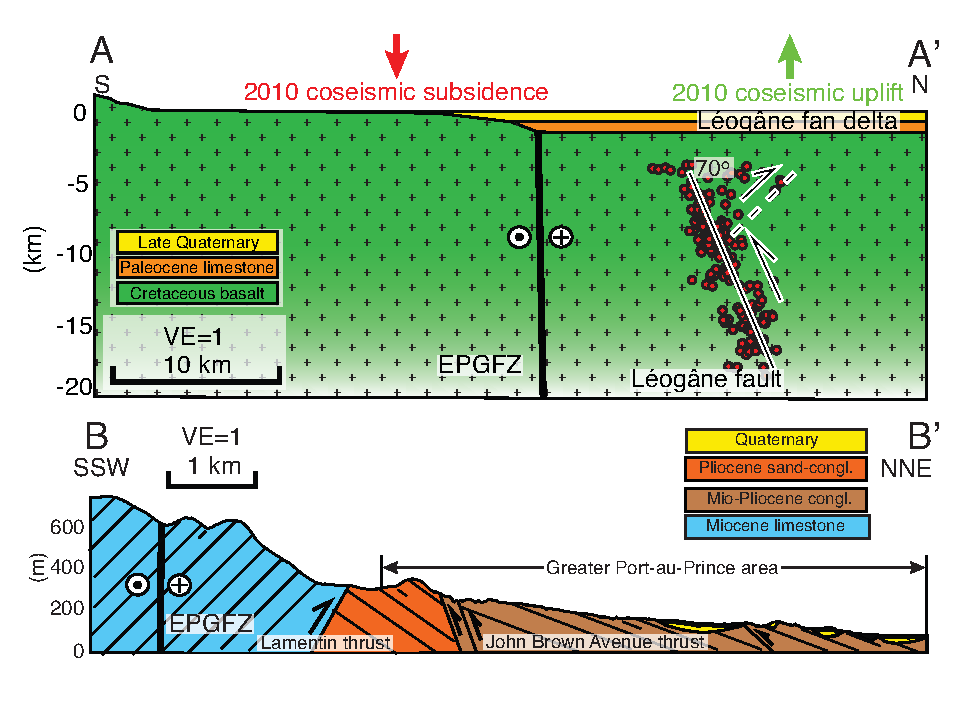
\includegraphics[width=\textwidth]{Haiti_figure3}
\caption{\textbf{Structure of the EPGFZ in the Mirago\^ane-L\'eog\^ane region. A:} Structure \citep{prentice2010seismic} and aftershock \citep{douilly2015three} map of Mirago\^ane-L\'eog\^ane region overlain with an InSAR image. \textbf{B:} Bathymetry of Lake Mirago\^ane in the two traces of the EPGFZ surface fracture map. \textbf{C:} Sonar profile M1. \textbf{D:} Sonar profile M5. \textbf{E:} Tie between chirp sonar and core \citep{higuera199910} extending to lacustrine sediments deformed by the EPGFZ at 1770. \textbf{F:} Low-pass filtered E/P log (red) and the synthetic sonar profile generated from the low-pass filtered E/P log used as an acoustic impedance. Red bar in the Figure~3C,D is the core measurement \citep{higuera199910} location.}
\label{figure3}
\end{figure}

\begin{figure}
\centering
\includegraphics[width=\textwidth]{figure4}
\caption{\textbf{Three-dimensional block diagram showing the structural and aftershock expression of late Holocene strain partitioning in a 40-km-wide zone along a 120 km-long segment of the EPGFZ.} Black arrows show southwest direction of the Gon\^ave microplate relative to the Caribbean plate and 2010 InSAR-derived surface deformation map show and large component of shortening accommodated on a 40-km-wide zone of oblique thrusts and folds north of the EPGFZ. PaP: Port-au-Prince; PG: Petit Goave; LA: Lake Azuey; LM: Lake Mirago\^ane-L\'eog\^ane; JF: Jimani thrust fault; LMF: Lamartin thrust fault; TBF: Trois Baies thrust fault; LF: L\'eog\^ane fault.}
\label{figure4}
\end{figure}

\end{document}
